This section focuses on introducing the proposed unsupervised hyperspectral image segmentation algorithm Adaptive Superpixel Cuts for Hyperspectral Images (ASC-HSI). This algorithm leverages the algorithms proposed in Section \ref{Background} to perform image segmentation on a superpixel-basis rather than a pixel-basis, reducing computational and memory costs while allowing for the use of a graph based approach to segmentation and unmixing. The steps of the algorithm can depicted as follows:
\begin{figure}[h]
    \centering % This centers the image
    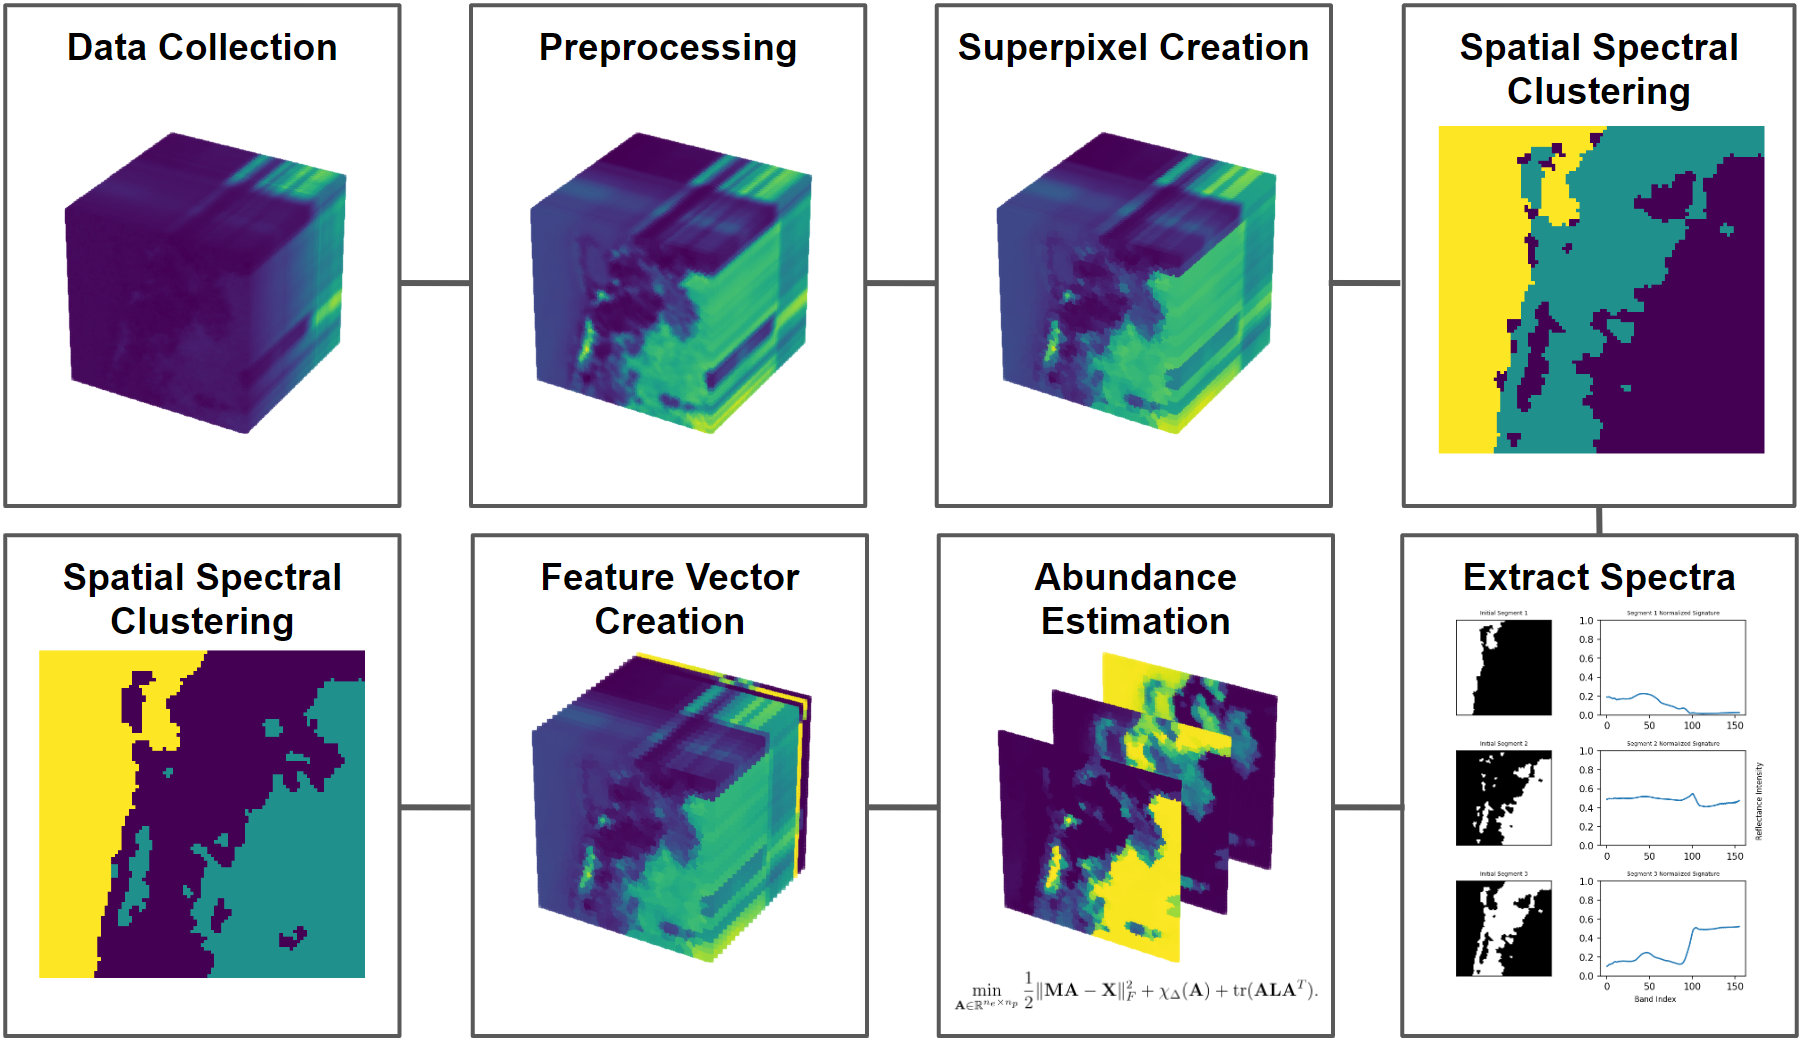
\includegraphics[scale=0.4]{algorithm_view.png}  % Replace filename with your image file name (without extension)
    \label{fig:label}  % Optional label for referencing the figure in the text
  \end{figure}
  
